%======================================================
% This file is part of
% "AMCOS_booklet"
% Version 1.1 (04/07/2019)
% A LaTeX template for conference books of abstracts
%
% This template is available at:
% https://github.com/maximelucas/AMCOS_booklet
%
% License: GNU General Public License v3.0
%
% Authors:
% Maxime Lucas (ml.maximelucas@gmail.com)
% Pau Clusella
%=======================================================

\documentclass[openany, parskip=full, 12pt, a4]{scrbook}

%======================================================
% This file is part of
% "AMCOS_booklet"
% Version 1.1 (04/07/2019)
% A LaTeX template for conference books of abstracts
%
% This template is available at:
% https://github.com/maximelucas/AMCOS_booklet
%
% License: GNU General Public License v3.0
%
% Authors:
% Maxime Lucas (ml.maximelucas@gmail.com)
% Pau Clusella
%=======================================================


\usepackage[utf8]{inputenc}
\usepackage[T1]{fontenc}


%---------------------------------------------------------
% PACKAGES
%---------------------------------------------------------

% TYPOGRAPHY
\usepackage{xspace}
\usepackage{microtype}
\usepackage{cmbright} % different fonts

% VARIA
\usepackage{color}
\usepackage[table]{xcolor} % loads also »colortbl« %load before tikz if options
\usepackage{scrhack} % fix koma script warning about addtolist
\usepackage{blindtext}
\usepackage{pdfpages} % for cover 

\usepackage{ifthen} % to have online and printed versions

% GRAPHICS & FIGURES & TABLES
\usepackage{graphicx}
\usepackage{float}
\usepackage{multicol} % for timetable
\usepackage{longtable} % for list of participants over more than 1 page
%\usepackage{wrapfig}
%\usepackage{tikz}
%\tikzset{ar/.style={>=latex, ->}}
%\renewcommand{\arraystretch}{1.2}
%\usepackage[multidot]{grffile}
% \usepackage{booktabs}

% WANTS TO BE LAST
\usepackage[portuguese]{babel}

\usepackage[hidelinks]{hyperref}
\hypersetup{pdfpagelayout=TwoPageRight}
% \usepackage[ocgcolorlinks]{hyperref}
% \hypersetup{colorlinks, linkcolor={wolf}, linktocpage=true, citecolor ={tpred}, urlcolor={black}}


%-------------------------------------------------------------
% SETTINGS
%-------------------------------------------------------------
\pagestyle{plain}

\setcounter{secnumdepth}{-2} % remove numbering at any level both for the heading and the toc
%https://tex.stackexchange.com/questions/30122/generate-table-of-contents-when-section-sections-without-numbering-has-been

%-------------------------------------------------------------
% USEFUL DEFINTIONS
%-------------------------------------------------------------

% VARIA 
\newcommand\tab[1][1cm]{\hspace*{#1}}
%======================================================
% This file is part of
% "AMCOS_booklet"
% Version 1.1 (04/07/2019)
% A LaTeX template for conference books of abstracts
%
% This template is available at:
% https://github.com/maximelucas/AMCOS_booklet
%
% License: GNU General Public License v3.0
%
% Authors:
% Maxime Lucas (ml.maximelucas@gmail.com)
% Pau Clusella
%=======================================================

%
% COLORS
%

\definecolor{myorange}{RGB}{255,117,40}
\definecolor{mygray}{RGB}{164, 168, 172}
\definecolor{mywhite}{RGB}{235, 238, 231}
\definecolor{myblue}{RGB}{38, 88, 89}
\definecolor{mygreen}{RGB}{128, 194, 61}

\newcommand{\primarycolor}{mygreen}
\newcommand{\secondarycolor}{myblue}
\newcommand{\ternarycolor}{mywhite}

%
% BOOKLET VERSIONS
%

% If compilation is done with 'compile.sh', both versions (online and printed) are automatically compiled
% If compilation is done from editor, choose which version to compile below
\makeatletter
\@ifundefined{ifOnline}{% % check if already defined from the command line, if not define \ifOnline
	\expandafter\newif\csname ifOnline\endcsname
	\Onlinetrue %set to \Onlinefalse/\Onlinetrue for printed/online version
}{}
\makeatother

% define \type to input the right version of the abstract
\ifOnline
\newcommand{\type}{o}
\else
\newcommand{\type}{p}
\fi % end if

%
% ABSTRACT ENVIRONMENTS
%

%----------------------------------------
% online abstract environment
%----------------------------------------
\newenvironment{abstract_online}[4] %{title}{author}{affiliation}{type}
{\filbreak %avoid page break
	
	{\large \bfseries #1}
	
	{\bfseries \itshape #2} \hfill {#3}
	
	\textcolor{mygray}{#4}
	
}
{}

%----------------------------------------
% talk abstract environment (printed)
%----------------------------------------
\newenvironment{abstract}[4] %{title}{author}{affiliation}
{\filbreak %avoid page break
	
	{\large \bfseries #1}
	
	{\bfseries \itshape #2,} \textcolor{mygray}{#3} \hfill {#4}
	
	
}
{}

%----------------------------------------
% poster abstract environment (printed)
%----------------------------------------
\newcommand{\poster}[3] %{title}{author}{affiliation}
{\filbreak %avoid page break
	
	{\bfseries \large #1} \\	
	\tab #2, \textit{#3}
	
}
{}

%----------------------------------------
% tags for talk type (colored circle in abstracts)
%----------------------------------------

\newcommand{\KLtag}{\tikz[baseline={([yshift=-.8ex]current bounding box.center)}]  \node[circle, inner sep=2pt, minimum size=0.5em, color=black, fill=\KLcolor]{\small \bfseries KL};} %colored circle with tag

\newcommand{\IStag}{\tikz[baseline={([yshift=-.8ex]current bounding box.center)}]  \node[circle, inner sep=2pt, minimum size=0.5em, color=black, fill=\IScolor]{\small \bfseries IS};} %colored circle with tag

\newcommand{\CTtag}{\tikz[baseline={([yshift=-.8ex]current bounding box.center)}]  \node[circle, inner sep=2pt, minimum size=0.5em, color=black, fill=\CTcolor]{\small \bfseries CT};} %colored circle with tag

\newcommand{\ITtag}{\tikz[baseline={([yshift=-.8ex]current bounding box.center)}]  \node[circle, inner sep=2pt, minimum size=0.5em, color=black, fill=\ITcolor]{\small \bfseries IT};} %colored circle with tag

%
% PAGE LAYOUT DEFINITIONS
%
\usepackage{etoolbox}

%------------------------------------------------------
% page style: vertical line on the side of each page
%------------------------------------------------------
\usepackage[scale=1,angle=0,opacity=1]{background}
\backgroundsetup{contents={}}

\AddEverypageHook{%
\ifthenelse{%
	\isodd{\thepage} \AND  \thepage>1 % if odd page but not front page
	}{%
	\backgroundsetup{
		color=\secondarycolor,
		position=current page.south east,%
		nodeanchor=south east,
		contents={\rule{10pt}{0.66\paperheight}}
		}
	}{%
	% nothing
	}
%
\ifthenelse{% 
	\NOT \isodd{\thepage} \AND \NOT \thepage=44% if even page
	}{%
	\backgroundsetup{
		color=\secondarycolor,
		position=current page.south west,%
		nodeanchor=south west,
		contents={\rule{10pt}{0.66\paperheight}}
		}
	}{%
	% nothing
	}
\BgMaterial}


%---------------------------------------------------
% chapter heading style
%---------------------------------------------------

\newdimen\mybarpadding
\mybarpadding=1.5em\relax %padding between gcolored bar and chapter name

\RedeclareSectionCommand[%
    ,afterskip=4em plus 1pt minus 1pt%
    ,beforeskip=-1pt%1.2em plus 1pt minus 1pt%
    ,level=0%
    ,toclevel=0%
]{chapter}%

\setkomafont{chapter}{\bfseries\Huge\color{myblue}} % 

\setkomafont{section}{\bfseries\Large\color{myblue}} % 
% koma-script-specific command

\newcommand*{\mynumberedtest}[1]{% to test whether there is a number
  \if\relax\detokenize{#1}\relax%
  \else%
    #1%
    
  \fi}


%-------------------------------------------------chapter style definition

\renewcommand{\chapterlinesformat}[3]{%
  \ifthispageodd{%
    \hfill%
    \raisebox{-0.2em}{%
      \makebox[0pt][r]{\textcolor{\primarycolor}{\rule{\paperwidth}{1em}}}%
    }%
    \hspace{\mybarpadding}%
% 	\mynumberedtest{#2}
	\mbox{#3}%
  }{%
%    \hbox{%
%       \mynumberedtest{#2}
      \mbox{#3}%
      \hspace{\mybarpadding}%
      \raisebox{-0.2em}{%
        \makebox[0pt][l]{\textcolor{\primarycolor}{\rule{\paperwidth}{1em}}}%
      }%
%    }%
  }%
}
\makeatother
%---------------------------------------------------------

% TIMETABLE COLORS AND STYLES

% text and backgroud colors
\newcommand{\tbg}{gray} % background
\newcommand{\tfg}{white}
\newcommand{\tbc}{gray!25}

% talk types colors
\newcommand{\IScolor}{myblue!65} % invited speaker
\newcommand{\CTcolor}{white} % contributed talk
\newcommand{\KLcolor}{myorange!45} % keynote lecture
\newcommand{\ITcolor}{yellow!25} %

% row types
\newcommand{\tablebreak}[2]{% {time span}{break name}
	\rowcolor{\tbc} #1 &  \multicolumn{4}{c|}{\bfseries #2} \\ \hline }
\newcommand{\eventtype}[2]{% {time span}{event name}
	#1& \multicolumn{4}{c|}{\cellcolor{\tbg}\color{\tfg}\bfseries #2} \\ \hline }

% column spacing and position
\newcolumntype{L}[1]{%
	>{\raggedright\let\newline\\\arraybackslash\hspace{0pt}}m{#1}}
\newcolumntype{C}[1]{%
	>{\centering\let\newline\\\arraybackslash\hspace{0pt}}m{#1}}
\newcolumntype{R}[1]{%
	>{\raggedleft\let\newline\\\arraybackslash\hspace{0pt}}m{#1}}

%\newcommand{\mytable}{|C{0.15\linewidth}| C{0.05\linewidth}|  C{0.25\linewidth} C{0.1\linewidth} C{0.5\linewidth}|}

\newcommand{\IS}[5]{% {time span}{name}{University}{City, Country}{title}
	#1 &\cellcolor{\IScolor}IS&{\bfseries#2}\newline #4&&#5 \\ \hline}
\newcommand{\CT}[5]{%
	#1 &\cellcolor{\CTcolor}CT&{\bfseries#2}\newline #4&&#5 \\ \hline}
\newcommand{\KL}[5]{%
	#1 &\cellcolor{\KLcolor}KL&{\bfseries#2}\newline #4&&#5 \\ \hline}
\newcommand{\IT}[5]{%
	#1 &\cellcolor{\ITcolor}IT&{\bfseries#2}\newline #4&&#5 \\ \hline}
\newcommand{\tutorial}[5]{%
	#1 && {\bfseries#2}\newline #4 &&#5 \\ \hline}
	
\begin{document}

% COVER PAGE
%--------------------------------------------------------------------
\includepdf{cover}	% our cover was produced with canva.com
	
	
% BLANK PAGE
%---------------------------------------------------------------------
\mbox{}
\thispagestyle{empty}
\vfill
\begin{center}
	\ifOnline
	A versão electrónica deste booklet pode ser descarregada em: \\
	https://apor.pt/
	\else
	This is the shor version of the booklet for print use. Full abstracts with all authors, references, and figures can be found in the electronic version at \url{https://amcosconference.com/}
	\fi % end if
	\\[20pt] % Please cite us by keeping the following line.
	The open-source \LaTeX{} template, AMCOS\_booklet, used to generate this booklet is available at \url{https://github.com/maximelucas/AMCOS\_booklet}
\end{center}

\newpage

% TABLE OF CONTENTS 
%---------------------------------------------------------------------
\tableofcontents

% ABOUT
%---------------------------------------------------------------------
\chapter{Acerca}

\section{XXIV Congresso Nacional de Ortoptistas - APOR}

O Congresso Nacional de Ortoptistas é organizado anualmente pela APOR - Associação Portuguesa de Ortoptistas, e segue na sua 24ª Edição. Conta com a participação de profissionais, estudantes e investigadores, e tem como objetivo a partilha de conhecimentos e experiências entre os profissionais da área da Ortóptica e ciências da visão, bem como a divulgação de trabalhos científicos e técnicos.

A APOR é uma associação profissional de direito privado, sem fins lucrativos, que tem como objetivo a promoção e desenvolvimento da profissão de Ortóptista em Portugal. Da sua missão fazem parte ainda a cooperação com outras associações e entidades nacionais e internacionais, a divulgação de informação científica e técnica, a promoção da formação e investigação científica assim como da qualidade dos cuidados de saúde prestados à população.

\section{Comissão Organizadora}
\begin{flushleft}
\begin{tabular}{lll}
Ana Maia & Carmen Oliveira &  Diana Silva \\
Dina Drogas & Diogo Marques &  Hugo Quental\\
João Ferreira & Maria Eduarda Lage & Nadine Gonçalves \\
Rodolfo Moura & Sandra Gonçalves 
\end{tabular}
\end{flushleft}

\section{Comissão Científica}
\begin{flushleft}
\begin{tabular}{l}
Ana Rita Santos, PhD, AIBILI, iCBR, ESS-IPP \\
Carla Lança, PhD, ESTeSL, CHRC ENSP-UNL \\
Catarina Mateus, PhD, T.BIO, ESS-IPP; CIBIT \\ 
Gonçalo Marques, MSc, IVLC, ESTeSL-IPL \\
Pedro Camacho, PhD, H\&TRC - ESTeSL, IPL; iNOVA4Health - FCM, UNL; IOGP \\ 
\end{tabular}
\end{flushleft}

% TIMETABLE 
%---------------------------------------------------------------------
\chapter{Agenda}

CO: Comunicação Oral, PC: Palestrante convidado, CP: Conferência Principal.
% Custom commands used here can be found at the end of the preamble_booklet.tex file

\section{Quinta-feira, 18 de abril}
\begin{center}
	\filbreak
\begin{longtable}{|C{0.15\linewidth}| C{0.04\linewidth}|  C{0.3\linewidth} C{0.0\linewidth} C{0.4\linewidth}|}\hline	
	\tablebreak{8:30--9:00}{Abertura do Secretariado}
	\eventtype{9:15--10:30}{Simpósio de farmacologia}
	\KL{}{André Coelho}{}{ESTeSL}{Farmacologia Ocular}
	\CT{}{Mara Ferreira}{}{H. Luz, APDP}{Medicação sistémica com repercussões oculares}
	\tablebreak{10:30--11:00}{Coffee-break e visita à exposição técnica}
	\IS{11:00--11:40}{Hiroya Sato}{}{Tokyo, Japan}{Title of invited speaker}
	\CT{11:40--12:45}{Marc Smith}{}{Brussels, Belgium}{Title of contributed talk with math and paragraphs}
	\tablebreak{12:00--13:30}{Almoço livre}
	\CT{14:00--14:30}{Marc Rodriguez}{}{Barcelona, Spain}{Title of contributed talk with math and references}
	\IS{14:30--15:05}{Hiroya Sato}{}{Tokyo, Japan}{Title of invited speaker}
	\tablebreak{15:05--15:30}{Coffee-break e visita à exposição técnica}
	\CT{15:30-16:00}{Marc Jansen}{}{Amsterdam, The Netherlands}{Title of contributed talk and references and a figure}
	\IS{16:00-17:10}{Hiroya Sato}{}{Tokyo, Japan}{Title of invited speaker}
	\eventtype{17:10--19:30}{Poster session with Wine \& Cheese}
\end{longtable}
\end{center}

\newpage
\section{Sexta-feira, 19 de abril}
\begin{center}
	\begin{longtable}{|C{0.15\linewidth}| C{0.04\linewidth}|  C{0.3\linewidth} C{0.0\linewidth} C{0.4\linewidth}|}\hline	
		\IS{9:00-9:40}{Hiroya Sato}{}{Tokyo, Japan}{Title of invited speaker}
		\CT{9:40-10:10}{Marc Fournier}{}{Brussels, Belgium}{Title of contributed talk}
		\IS{10:10--12:45}{Hiroya Sato}{}{Tokyo, Japan}{Title of invited speaker}
		\tablebreak{10:30--11:00}{Coffee-break e sessão de posters}
		%odor
		\CT{11:10--11:40}{Marc Jansen}{}{Amsterdam, The Netherlands}{Title of contributed talk and references and a figure}
		\CT{11:40--12:10}{Marc Jansen}{}{Amsterdam, The Netherlands}{Title of contributed talk and references and a figure}
		\IS{12:10--12:45}{Hiroya Sato}{}{Tokyo, Japan}{Title of invited speaker}
		\tablebreak{12:45--14:00}{Almoço livre}
		\CT{14:00--14:30}{Marc Fournier}{}{Brussels, Belgium}{Title of contributed talk}
		\CT{14:30-15:00}{Marc Fournier}{}{Brussels, Belgium}{Title of contributed talk}
		\eventtype{16:30--18:00}{Excursion}
		\eventtype{20:00}{Conference Dinner}
	\end{longtable}
\end{center}

\newpage
\section{Sábado, 20 de abril}
\begin{center}
	\begin{longtable}{|C{0.15\linewidth}| C{0.04\linewidth}|  C{0.3\linewidth} C{0.0\linewidth} C{0.4\linewidth}|}\hline	
		\IS{9:00 -- 9:40}{Hiroya Sato}{}{Tokyo, Japan}{Title of invited speaker}
		\IS{9:40--10:20}{Hiroya Sato}{}{Tokyo, Japan}{Title of invited speaker}
		\IT{10:20--10:45}{Franck Schmidt}{}{Munich, Germany}{A Special Talk about Diversity in Science}
		\tablebreak{10:45--11:10}{Coffee}
		\CT{11:10-11:40}{Marc Jansen}{}{Amsterdam, The Netherlands}{Title of contributed talk and references and a figure}
		\KL{11:40--12:35}{Leon Tremblay}{}{Montreal, Canada}{Title of a keynote lecture}
		\eventtype{12:35--12:45}{Poster Prize \& Conclusion}
		\tablebreak{12:45--14:00}{Almoço livre}
	\end{longtable}
\end{center}


% TALKS 
%---------------------------------------------------------------------
\chapter{Resumos -- Comunicações Orais}

\section{Quinta-feira, 18 de abril}

% Definitions of custom environment used here can be found in preamble_booklet.tex file

% The following input commands automatically select the right version 
% (print or online) version of the abstract's .tex
% \type is defined in preamble_booklet.tex and equals:
% 'o' (online) or 'p' (print)

\input{abstracts/tex/t\type_tremblay}

\section{Sexta-feira, 19 de abril}

\section{Sábado, 20 de abril}

% POSTERS
%------------------------------------------------------------------
\chapter{Resumos -- Posters} 

\vspace{-2.5em}

\section{Sessão de apresentação, 19 de abril}

\input{abstracts/tex/p\type_pocas}


% LIST OF PARTICIPANTS
%------------------------------------------------------------------
\chapter{Índice de participantes}
 
\input{list_of_participants}
 
% USEFUL INFO
%------------------------------------------------------------------
\chapter{Informações úteis}

\textbf{Talks} will be held at the \textbf{Conference Hall-Auditorium} of PRBB. It is situated on the first floor of the central courtyard and
has independent access from the rest of the building (through stairs located at the ground floor, main entrance of PRBB). 

A \textbf{sessão de posters} terá lugar na sexta-feira, simultaneamente com a pausa para coffee-break da manhã (10h30) junto do \textbf{hall da exposição técnica}. Deverá ser garantida a presença de pelo menos um dos autores durante a sessão para discussão dos trabalhos.

Rede wi-fi será disponibilizada no local do evento.

O \textbf{jantar convívio} terá lugar no Restaurante Waikiki às Xh, na morada.

\section{Como chegar ao Congresso?}



\begin{itemize}

	\item \textbf{Subway:} yellow line, L4, station Ciutadella/Vila Ol\'{i}mpica,
	\item \textbf{Bus:} lines V21, 14, 36, 41, 45, 59, 71, 92, D20,
	\item \textbf{Tram:} line 4, stop Vila Ol\'{i}mpica.
	
\end{itemize}

\begin{center}
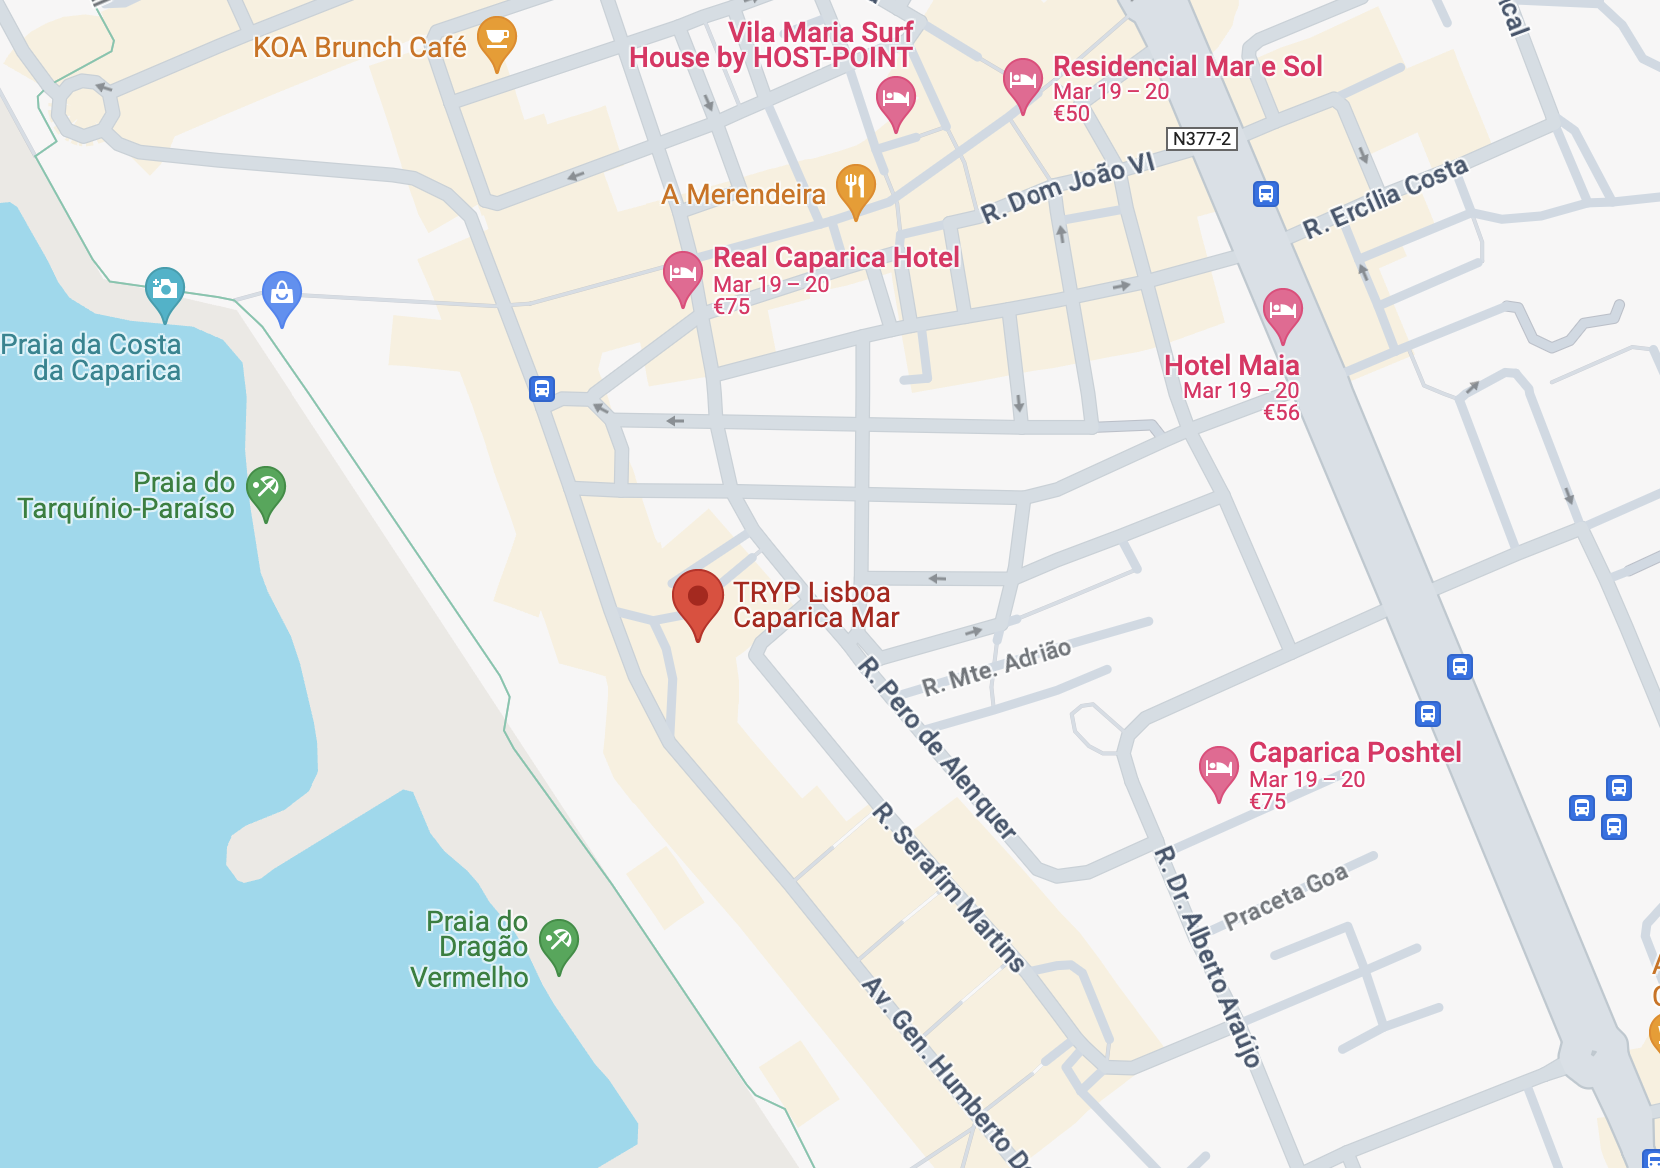
\includegraphics[width=\linewidth]{images/tryp_map}
\end{center}


% SPONSORS
%------------------------------------------------------------------
\chapter{Parceiros}

\begin{center}
The AMCOS conference is part of the COSMOS project, funded by the European Union’s Horizon 2020 research and innovation programme under the Marie Sk\l{}odowska-Curie grant agreement No 642563.
\end{center}

\vfill

\section{Com o apoio de:}

\begin{center}
\includegraphics[width=0.5\textwidth]{images/logos/Partnerlogos/LancasterHelium.jpg}
%\includegraphics[width=0.5\textwidth]{images/logos/Partnerlogos/springer.pdf}
\end{center}

\vfill

\newpage

% BACK PAGE
%-----------------------------------------------------------------

\pagecolor{myblue}
\thispagestyle{empty}
\mbox{}

\end{document}
